\documentclass[aspectratio=169, 11pt]{beamer}

% =====================================================================
%  Theme & styling --- matches the minor presentation
% =====================================================================
\usetheme{Madrid}
\usecolortheme{default}

\definecolor{iiitmblue}{RGB}{0, 70, 140}
\definecolor{iiitmlight}{RGB}{220, 235, 250}
\definecolor{accentgreen}{RGB}{34, 139, 34}
\definecolor{accentred}{RGB}{180, 30, 30}
\definecolor{accentamber}{RGB}{210, 140, 0}

\setbeamercolor{palette primary}{bg=iiitmblue, fg=white}
\setbeamercolor{palette secondary}{bg=iiitmblue!80, fg=white}
\setbeamercolor{palette tertiary}{bg=iiitmblue!60, fg=white}
\setbeamercolor{structure}{fg=iiitmblue}
\setbeamercolor{title}{fg=white, bg=iiitmblue}
\setbeamercolor{frametitle}{fg=white, bg=iiitmblue}
\setbeamercolor{block title}{bg=iiitmblue, fg=white}
\setbeamercolor{block body}{bg=iiitmlight, fg=black}
\setbeamercolor{block title alerted}{bg=accentred, fg=white}
\setbeamercolor{block body alerted}{bg=red!5, fg=black}
\setbeamercolor{block title example}{bg=accentgreen, fg=white}
\setbeamercolor{block body example}{bg=green!5, fg=black}
\setbeamercolor{item}{fg=iiitmblue}

\setbeamertemplate{navigation symbols}{}
\setbeamertemplate{footline}{%
  \leavevmode%
  \hbox{%
    \begin{beamercolorbox}[wd=.35\paperwidth,ht=2.5ex,dp=1ex,center]{palette primary}%
      \usebeamerfont{author in head/foot}\insertshortauthor
    \end{beamercolorbox}%
    \begin{beamercolorbox}[wd=.40\paperwidth,ht=2.5ex,dp=1ex,center]{palette secondary}%
      \usebeamerfont{title in head/foot}\insertshorttitle
    \end{beamercolorbox}%
    \begin{beamercolorbox}[wd=.25\paperwidth,ht=2.5ex,dp=1ex,right]{palette tertiary}%
      \usebeamerfont{date in head/foot}%
      \insertframenumber{} / \inserttotalframenumber\hspace*{2ex}
    \end{beamercolorbox}%
  }%
  \vskip0pt%
}

% =====================================================================
%  Packages
% =====================================================================
\usepackage[utf8]{inputenc}
\usepackage[T1]{fontenc}
\usepackage{lmodern}
\usepackage{amsmath}
\usepackage{booktabs}
\usepackage{tikz}
\usepackage{pgfplots}
\pgfplotsset{compat=1.18}
\usepackage{listings}
\usepackage{graphicx}
\usetikzlibrary{shapes.geometric, arrows.meta, positioning, calc}

\lstdefinestyle{beamerstyle}{
    basicstyle=\ttfamily\scriptsize,
    keywordstyle=\color{iiitmblue}\bfseries,
    commentstyle=\color{gray},
    stringstyle=\color{accentgreen},
    backgroundcolor=\color{iiitmlight},
    frame=single,
    rulecolor=\color{iiitmblue!30},
    breaklines=true,
    showstringspaces=false,
    tabsize=2,
}
\lstset{style=beamerstyle}

% =====================================================================
%  Meta
% =====================================================================
\title[BTP End-Term]{Reducing Cross-Node Network Calls in\\Distributed Payment Systems}
\subtitle{B.Tech Project --- End-Term Evaluation\\\small with Concurrency-Safe Resolution of Single-Resource Contention}
\author[Raman Kapoor]{Raman Kapoor}
\institute[ABV-IIITM]{ABV --- Indian Institute of Information Technology\\and Management, Gwalior\\[0.5em]\textbf{Supervisor:} Dr.\ Rahul Kala}
\date{2026}

% =====================================================================
\begin{document}

% ---------- Slide 1: Title ----------
{
\setbeamertemplate{footline}{}
\begin{frame}
\titlepage
\end{frame}
}

% ---------- Slide 2: Outline ----------
\begin{frame}{Outline}
\tableofcontents
\end{frame}

% ============================================================
\section{Motivation}
% ============================================================

\begin{frame}{The Problem We Started With}
\begin{block}{Distributed payments at scale}
\begin{itemize}
    \item $\sim$68{,}000 cross-node operations per second
    \item Each request triggers \textbf{5--15 cross-node calls}
    \item p95 = 98\,ms, p99 = 285\,ms at peak
    \item Strict correctness: every transaction must be exactly once
\end{itemize}
\end{block}
\pause
\begin{alertblock}{Tension}
Aggressive caching reduces latency \textbf{but} risks staleness, lost updates, and double-allocation in a financial system.
\end{alertblock}
\end{frame}

\begin{frame}{What the Minor Established}
\begin{itemize}
    \item Two-tier in-process caching (thread + server-local) is \textbf{safe} for configuration-class data
    \item Formal cache-safety boundary framework (4 criteria)
    \item Phase 1 results in production:
    \begin{itemize}
        \item \textbf{4.1\%} cross-node call reduction at peak
        \item \textbf{--11.2\%} p95, \textbf{--13.0\%} p99 API latency
        \item \textbf{--26.2\%} Redis p99 latency
        \item Zero correctness incidents
    \end{itemize}
\end{itemize}
\pause
\begin{alertblock}{Open question raised at the minor evaluation}
\centering
\emph{``If you cache state, how do you prevent two users from booking the same single piece?''}
\end{alertblock}
\end{frame}

\begin{frame}{This is the Question We Answer}
\begin{exampleblock}{End-term contribution}
A \textbf{contention layer} that composes with the cache and provably prevents double-allocation on single, indivisible resources --- inventory units, reservation slots, account balances, gateway tokens.
\end{exampleblock}
\vspace{0.5em}
\textbf{Five complementary primitives:}
\begin{enumerate}
    \item Distributed locking with fencing tokens
    \item Atomic decrement via Redis Lua scripts
    \item Optimistic concurrency control (versioned cache)
    \item PN-Counter CRDTs (eventually consistent)
    \item Single-flight request coalescing
\end{enumerate}
\end{frame}

% ============================================================
\section{Two-Tier Caching: Recap}
% ============================================================

\begin{frame}{Two-Tier Cache --- Quick Recap}
\begin{columns}[T, onlytextwidth]
\column{0.50\textwidth}
\textbf{Tier 1: Thread-level}
\begin{itemize}
    \item \texttt{IORef HashMap}, per-request
    \item Destroyed on request end
    \item \textbf{Zero staleness} guarantee
    \item Hit rate: 22.3\%
\end{itemize}
\column{0.50\textwidth}
\textbf{Tier 2: Server-local}
\begin{itemize}
    \item \texttt{TVar} + LRU + TTL
    \item Shared across threads on a node
    \item TTLs: 30--120\,s by data class
    \item Hit rate: 41.7\%
\end{itemize}
\end{columns}
\vspace{0.6em}
\begin{block}{Cache-safety boundaries (must hold for cache-eligibility)}
\small
1. Immutability within TTL \quad
2. Request-scope independence \\
3. Idempotency of stale reads \quad
4. Deterministic key
\end{block}
\end{frame}

\begin{frame}{Why Caching Alone Is Not Enough}
\textbf{Single-resource state fails criterion (3):} a stale read can lead to double-allocation.
\vspace{0.5em}
\begin{center}
\resizebox{0.9\textwidth}{!}{%
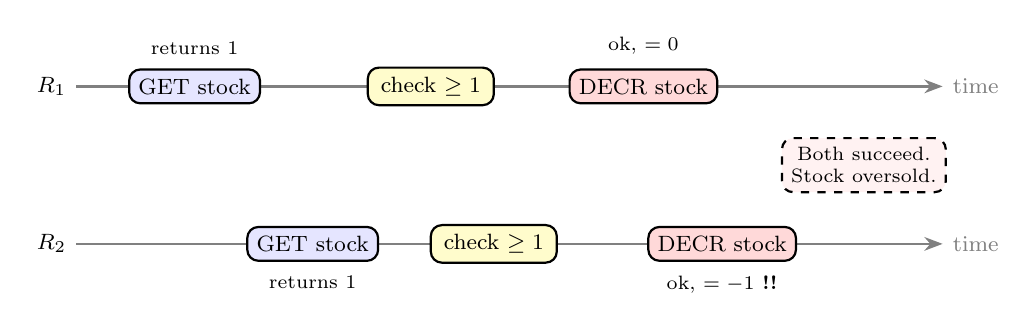
\begin{tikzpicture}[>=Stealth, thick, every node/.style={font=\footnotesize}]
    \draw[->, gray] (0,2) -- (11,2) node[right]{time};
    \draw[->, gray] (0,0) -- (11,0) node[right]{time};
    \node[left] at (0,2) {$R_1$};
    \node[left] at (0,0) {$R_2$};

    \node[draw, fill=blue!10, rounded corners, minimum width=1.6cm] (a) at (1.5,2) {GET stock};
    \node[font=\scriptsize, above=0.05cm of a] {returns 1};
    \node[draw, fill=blue!10, rounded corners, minimum width=1.6cm] (b) at (3.0,0) {GET stock};
    \node[font=\scriptsize, below=0.05cm of b] {returns 1};
    \node[draw, fill=yellow!20, rounded corners, minimum width=1.6cm] at (4.5,2) {check $\geq 1$};
    \node[draw, fill=yellow!20, rounded corners, minimum width=1.6cm] at (5.3,0) {check $\geq 1$};
    \node[draw, fill=red!15, rounded corners, minimum width=1.7cm] (d) at (7.2,2) {DECR stock};
    \node[font=\scriptsize, above=0.05cm of d] {ok, $=0$};
    \node[draw, fill=red!15, rounded corners, minimum width=1.7cm] (e) at (8.2,0) {DECR stock};
    \node[font=\scriptsize, below=0.05cm of e] {ok, $=-1$ \textbf{!!}};

    \node[draw, dashed, fill=red!5, rounded corners, align=center, font=\scriptsize] at (10,1) {Both succeed.\\Stock oversold.};
\end{tikzpicture}%
}
\end{center}
\textbf{The contention layer must close every variant of this race.}
\end{frame}

% ============================================================
\section{The Contention Layer: Five Primitives}
% ============================================================

\begin{frame}[fragile]{Primitive 1 --- Distributed Locking with Fencing Tokens}
\begin{itemize}
    \item Acquire a per-resource lock (Redlock on Redis, etcd lease) before read-modify-write
    \item \textbf{Fence token:} monotonically increasing number returned with the lock; backend rejects stale-token writes
    \item Mitigates GC pauses, partitions, clock drift
\end{itemize}
\begin{block}{Sketch}
\begin{lstlisting}[language=Haskell]
withLock conn key ttl $ \tok -> do
  v   <- backendRead key
  v'  <- compute v
  backendWriteIfFence key v' tok   -- backend checks tok
\end{lstlisting}
\end{block}
\textbf{Use when:} business logic is non-trivial; contention is moderate; the critical section calls external services.
\end{frame}

\begin{frame}[fragile]{Primitive 2 --- Atomic Decrement via Redis Lua}
\textbf{Idea:} package the entire ``check + decrement'' in one Lua script. Redis runs scripts atomically.
\begin{block}{Lua}
\begin{lstlisting}[language={[5.2]Lua}]
local a = tonumber(redis.call('GET', KEYS[1]) or '0')
local w = tonumber(ARGV[1])
if a >= w then
  redis.call('DECRBY', KEYS[1], w)
  return {1, a - w}
else
  return {0, a}
end
\end{lstlisting}
\end{block}
\begin{itemize}
    \item Latency: $<$1\,ms; throughput: $>10^5$ scripts/s/shard
    \item Cache: \textbf{display reads} stay cached; \textbf{authoritative decrement} bypasses cache and publishes invalidation
    \item Limitation: critical section must fit in a Lua script (no external calls)
\end{itemize}
\end{frame}

\begin{frame}[fragile]{Primitive 3 --- OCC with Versioned Cache Entries}
\begin{itemize}
    \item Each cache entry carries a version
    \item Reader records the version; writer issues a CAS (\texttt{WHERE version = ?})
    \item Conflict $\Rightarrow$ retry
\end{itemize}
\begin{block}{SQL form}
\begin{lstlisting}[language=SQL]
UPDATE inventory
   SET stock = stock - 1, version = version + 1
 WHERE sku = $1 AND version = $2 AND stock >= 1
RETURNING stock, version;
\end{lstlisting}
\end{block}
\textbf{Use when:} contention is rare (e.g.\ control-plane writes). \\
\textbf{Avoid when:} contention is high --- retry storms collapse throughput.
\end{frame}

\begin{frame}{Primitive 4 --- PN-Counter CRDTs}
\begin{itemize}
    \item Two grow-only counters per replica: $P_i$ (positive), $N_i$ (negative)
    \item Value $= \sum_i P_i - \sum_i N_i$; merge by element-wise max
    \item Writes are \textbf{local}, never blocked, eventually converge
\end{itemize}
\begin{exampleblock}{When to use}
Soft holds, cart abandonment counters, flash sales advertising ``$\sim$1{,}000 units'' --- where a small overshoot is business-acceptable.
\end{exampleblock}
\begin{alertblock}{When not to use}
Hard limits where every unit must be exact. CRDTs trade hard upper bounds for availability.
\end{alertblock}
\end{frame}

\begin{frame}{Primitive 5 --- Single-Flight (Request Coalescing)}
\textbf{Idea:} on a cache miss, only the \textbf{first} request fetches; concurrent requests for the same key wait on the leader's promise.
\begin{block}{Effect}
\begin{itemize}
    \item Collapses the \emph{front} of the contention curve
    \item One backend call instead of $k$ identical ones
    \item Tames cache stampedes / thundering herds
\end{itemize}
\end{block}
\begin{alertblock}{Important}
Single-flight \textbf{deduplicates} on a single node; it is \textbf{not} a substitute for atomicity. Compose it with Primitive~2 (Lua) for full safety across nodes.
\end{alertblock}
\end{frame}

% ============================================================
\section{Hybrid Architecture}
% ============================================================

\begin{frame}{Putting It Together}
\begin{center}
\resizebox{0.95\textwidth}{!}{%
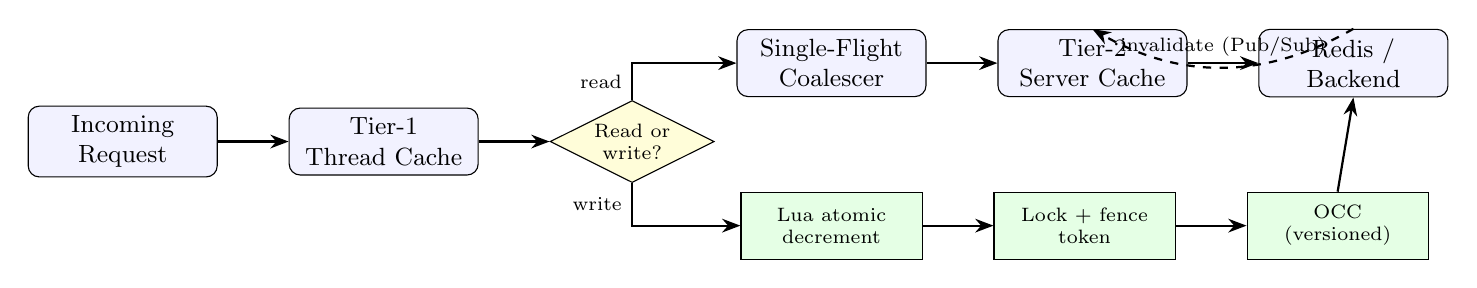
\begin{tikzpicture}[
    node distance=0.7cm and 0.9cm,
    box/.style={rectangle, draw, rounded corners, minimum height=0.85cm, minimum width=2.4cm, align=center, font=\small, fill=blue!5},
    decision/.style={diamond, draw, aspect=2, inner sep=1pt, align=center, font=\scriptsize, fill=yellow!15},
    primitive/.style={rectangle, draw, minimum height=0.85cm, minimum width=2.3cm, align=center, font=\scriptsize, fill=green!10},
    arrow/.style={-Stealth, thick}
]
    \node[box] (req) {Incoming\\Request};
    \node[box, right=of req] (t1) {Tier-1\\Thread Cache};
    \node[decision, right=of t1] (op) {Read or\\write?};

    \node[box, above right=0.3cm and 0.8cm of op] (sf) {Single-Flight\\Coalescer};
    \node[box, right=of sf] (t2) {Tier-2\\Server Cache};
    \node[box, right=of t2] (redis) {Redis /\\Backend};

    \node[primitive, below=1.2cm of sf] (lua) {Lua atomic\\decrement};
    \node[primitive, right=of lua] (lock) {Lock + fence\\token};
    \node[primitive, right=of lock] (occ) {OCC\\(versioned)};

    \draw[arrow] (req) -- (t1);
    \draw[arrow] (t1) -- (op);
    \draw[arrow] (op.north) |- node[pos=0.25, left, font=\scriptsize]{read} (sf.west);
    \draw[arrow] (op.south) |- node[pos=0.25, left, font=\scriptsize]{write} (lua.west);
    \draw[arrow] (sf) -- (t2);
    \draw[arrow] (t2) -- (redis);
    \draw[arrow] (lua.east) -- (lock.west);
    \draw[arrow] (lock.east) -- (occ.west);
    \draw[arrow] (occ.north) -- (redis.south);
    \draw[arrow, dashed] (redis.north) to[bend left=30] node[above, font=\scriptsize]{invalidate (Pub/Sub)} (t2.north);
\end{tikzpicture}%
}
\end{center}
\textbf{Reads} go through cache + single-flight. \\
\textbf{Authoritative writes} bypass the cache and select a primitive per data class.
\end{frame}

\begin{frame}{Decision Matrix}
\centering
\footnotesize
\setlength{\tabcolsep}{4pt}
\renewcommand{\arraystretch}{1.15}
\resizebox{0.95\textwidth}{!}{%
\begin{tabular}{p{3.0cm}p{1.6cm}p{2.4cm}p{2.0cm}p{2.6cm}}
\toprule
\textbf{Data class} & \textbf{Cache?} & \textbf{Primary} & \textbf{Coalescing} & \textbf{Notes} \\
\midrule
Merchant config (read)   & Tier-2  & ---              & Single-flight & Cache-eligible \\
Routing table (read)     & Tier-2  & ---              & Single-flight & Cache-eligible \\
Feature flag (read)      & Tier-2  & ---              & Single-flight & Cache-eligible \\
Inventory (display)      & Tier-2  & ---              & Single-flight & Approximate \\
Inventory (decrement)    & No      & Lua atomic       & Single-flight & Hard limit \\
Account balance debit    & No      & Distributed lock & Single-flight & Fence token \\
Reservation slot         & No      & Lua atomic       & Single-flight & Per-slot key \\
Soft hold (cart)         & Tier-2  & PN-Counter       & ---           & Over-alloc OK \\
Merchant config (write)  & Inval.  & OCC versioned    & ---           & Low contention \\
\bottomrule
\end{tabular}%
}
\end{frame}

\begin{frame}{Comparison of the Five Primitives}
\centering
\footnotesize
\setlength{\tabcolsep}{3pt}
\renewcommand{\arraystretch}{1.15}
\resizebox{\textwidth}{!}{%
\begin{tabular}{p{3.2cm}p{1.7cm}p{2.0cm}p{2.4cm}p{1.5cm}p{2.0cm}}
\toprule
\textbf{Property} & \textbf{Lock} & \textbf{Lua} & \textbf{OCC} & \textbf{CRDT} & \textbf{Single-flight} \\
\midrule
Hard upper bound          & Yes              & Yes                  & Yes                    & No        & N/A \\
Per-key throughput        & Low              & Very high            & Medium--high           & Very high & N/A \\
Latency overhead          & 1--3\,ms         & $<$1\,ms             & $<$1\,ms               & 0\,ms     & 0--1\,ms \\
Behaviour under partition & Blocks/fails     & Fails fast           & Fails fast             & Continues & Continues \\
Expressiveness            & High             & Lua only             & SQL/CAS                & Counter   & N/A \\
Composes with cache       & Bypass           & Bypass + invalidate  & Versioned cache        & Cached    & Front of cache \\
\bottomrule
\end{tabular}%
}
\end{frame}

% ============================================================
\section{Evaluation}
% ============================================================

\begin{frame}{Tail-Latency Reductions (Phase 1)}
\centering
\resizebox{0.85\textwidth}{!}{%
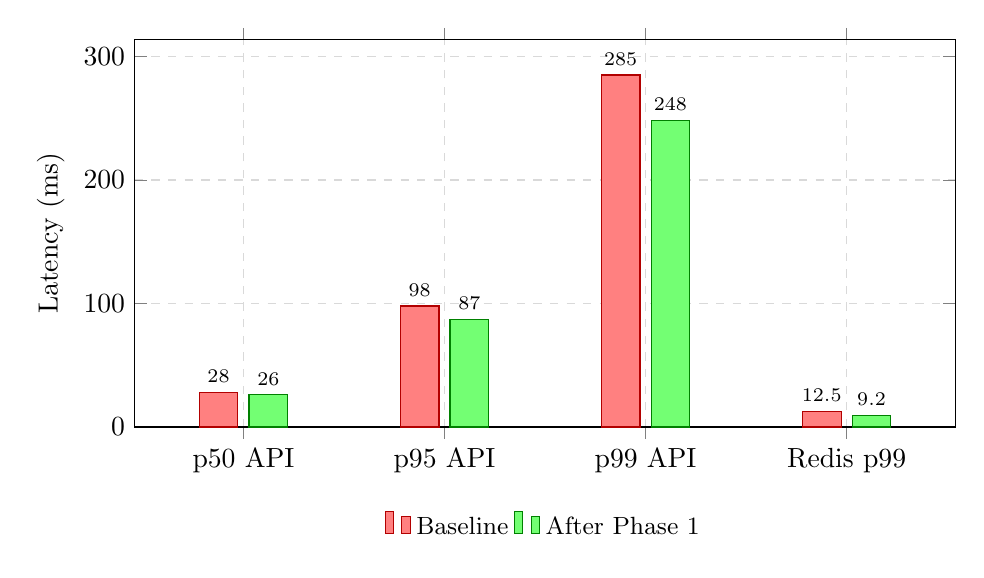
\begin{tikzpicture}
\begin{axis}[
    ybar=4pt, bar width=14pt,
    width=12cm, height=6.5cm,
    enlarge x limits=0.18,
    ylabel={Latency (ms)},
    xtick={1,2,3,4},
    xticklabels={p50 API, p95 API, p99 API, Redis p99},
    nodes near coords, nodes near coords style={font=\scriptsize},
    ymin=0,
    legend style={at={(0.5,-0.20)}, anchor=north, legend columns=2, font=\small, draw=none},
    grid=major, grid style={dashed, gray!30}
]
\addplot[fill=red!50!white, draw=red!70!black]    coordinates {(1,28) (2,98) (3,285) (4,12.5)};
\addplot[fill=green!55!white, draw=green!50!black] coordinates {(1,26) (2,87) (3,248) (4,9.2)};
\legend{Baseline, After Phase 1}
\end{axis}
\end{tikzpicture}%
}
\end{frame}

\begin{frame}{Cache Hit-Rate Breakdown}
\centering
\resizebox{0.78\textwidth}{!}{%
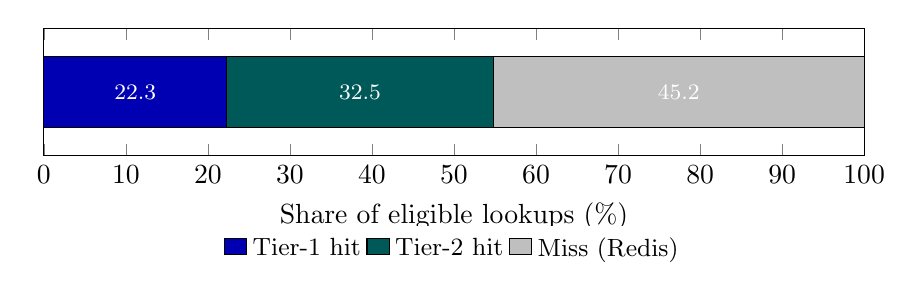
\begin{tikzpicture}
\begin{axis}[
    xbar stacked, width=12cm, height=3.2cm,
    xmin=0, xmax=100, xlabel={Share of eligible lookups (\%)},
    ytick=\empty, bar width=0.9cm,
    nodes near coords, nodes near coords style={font=\footnotesize, white},
    legend style={at={(0.5,-0.55)}, anchor=north, legend columns=3, font=\small, draw=none}
]
\addplot[fill=blue!70!black] coordinates {(22.3,0)};
\addplot[fill=teal!70!black] coordinates {(32.5,0)};
\addplot[fill=gray!50]       coordinates {(45.2,0)};
\legend{Tier-1 hit, Tier-2 hit, Miss (Redis)}
\end{axis}
\end{tikzpicture}%
}
\vspace{0.4em}
\begin{itemize}
    \item Combined hit rate \textbf{54.8\%} on eligible lookups
    \item $\sim$2{,}800 cross-node calls/sec eliminated cluster-wide
\end{itemize}
\end{frame}

\begin{frame}{Phase 2: Contention Layer in Production (30 days)}
\centering
\footnotesize
\setlength{\tabcolsep}{6pt}
\renewcommand{\arraystretch}{1.2}
\resizebox{\textwidth}{!}{%
\begin{tabular}{p{4.3cm}p{4.2cm}p{3.0cm}p{1.8cm}}
\toprule
\textbf{Workload} & \textbf{Primitive} & \textbf{Contention rate} & \textbf{p95 added} \\
\midrule
Inventory decrement (flash sale) & Lua + single-flight          & 1{,}400 contended/s & 0.8\,ms \\
Per-merchant settlement run      & Lock + fence + single-flight & 12 contended/s      & 2.6\,ms \\
Reservation slot booking         & Lua + single-flight          & 320 contended/s     & 1.1\,ms \\
Cart soft hold                   & PN-Counter (no coord.)       & N/A                 & 0.0\,ms \\
\bottomrule
\end{tabular}%
}
\vspace{0.6em}
\begin{exampleblock}{Correctness}
\begin{itemize}
    \item \textbf{Zero} double-allocation incidents
    \item \textbf{Zero} cache-related financial discrepancies
    \item Soft-hold over-allocation: 4.7 units/day on a 100k base ($<$1\% tolerance)
\end{itemize}
\end{exampleblock}
\end{frame}

% ============================================================
\section{Conclusion \& Future Work}
% ============================================================

\begin{frame}{Conclusion}
\begin{block}{What we built}
An integrated two-layer system: a \textbf{caching layer} for read-side latency reduction and a \textbf{contention layer} that closes the single-resource race the minor evaluation surfaced.
\end{block}
\begin{itemize}
    \item Cache-safety framework formalises which data is safe to cache
    \item Five contention primitives, each with a clear use case
    \item Decision matrix selects the right primitive per data class
    \item No new infrastructure beyond existing Redis cluster
\end{itemize}
\begin{exampleblock}{Headline numbers}
\centering
\textbf{--11.2\% p95}, \textbf{--13.0\% p99}, \textbf{--26.2\% Redis p99}, \\
\textbf{4.1\%} cross-node calls eliminated, \textbf{zero} correctness incidents.
\end{exampleblock}
\end{frame}

\begin{frame}{Future Work}
\begin{itemize}
    \item \textbf{Adaptive TTLs} that shrink under detected mutation pressure
    \item \textbf{Learned contention prediction} --- pre-warm the right primitive before flash sales
    \item \textbf{Verified fencing} --- TLA$^+$ / Coq mechanisation of the safety argument
    \item \textbf{Cross-DC extension} --- geo-replicated Redis vs.\ leader-elected coordinators
    \item \textbf{Graceful degradation modes} when Redis is partially unavailable
\end{itemize}
\end{frame}

\begin{frame}{Selected References (2024+)}
\footnotesize
\begin{itemize}
    \item Kumar et al., \emph{Comparative Analysis of Distributed Caching Algorithms}, arXiv:2504.02220, 2024.
    \item Wang et al., \emph{OptiQL: Robust Optimistic Locking for Memory-Optimised Indexes}, SIGMOD 2024.
    \item Wei et al., \emph{Motor: Multi-Versioning for Distributed Transactions on Disaggregated Memory}, OSDI 2024.
    \item Zhou et al., \emph{Concurrency Control as a Service}, VLDB 2025.
    \item \emph{Distributed Locking: Performance Analysis and Optimisation Strategies}, arXiv:2504.03073, 2025.
    \item Duncan, \emph{The CRDT Dictionary}, 2025.
    \item Redis Ltd., \emph{Reserve Inventory in Real Time with Redis (WATCH/MULTI)}, 2024.
\end{itemize}
\end{frame}

\begin{frame}
\begin{center}
{\Huge\bfseries Thank You}\\[1em]
{\Large Questions?}\\[2em]
{\small Raman Kapoor \quad $\bullet$ \quad ABV-IIITM Gwalior \quad $\bullet$ \quad 2026}
\end{center}
\end{frame}

\end{document}
